\section{Downsampling}
The digit data is stored at 300, 200 and 100 DPI.
The choice of pixel density is a tradeoff between
algorithm running times and classification accuracy.
With data from G2M2, k-NN prediction running times
were measured vs. dataset size N at various DPI.
The results
are presented in figure \ref{fig:knn-runningtime-vs-n-and-k}.
\begin{figure}[ht]
	\centering
	\begin{subfigure}[t]{0.33\textwidth}
		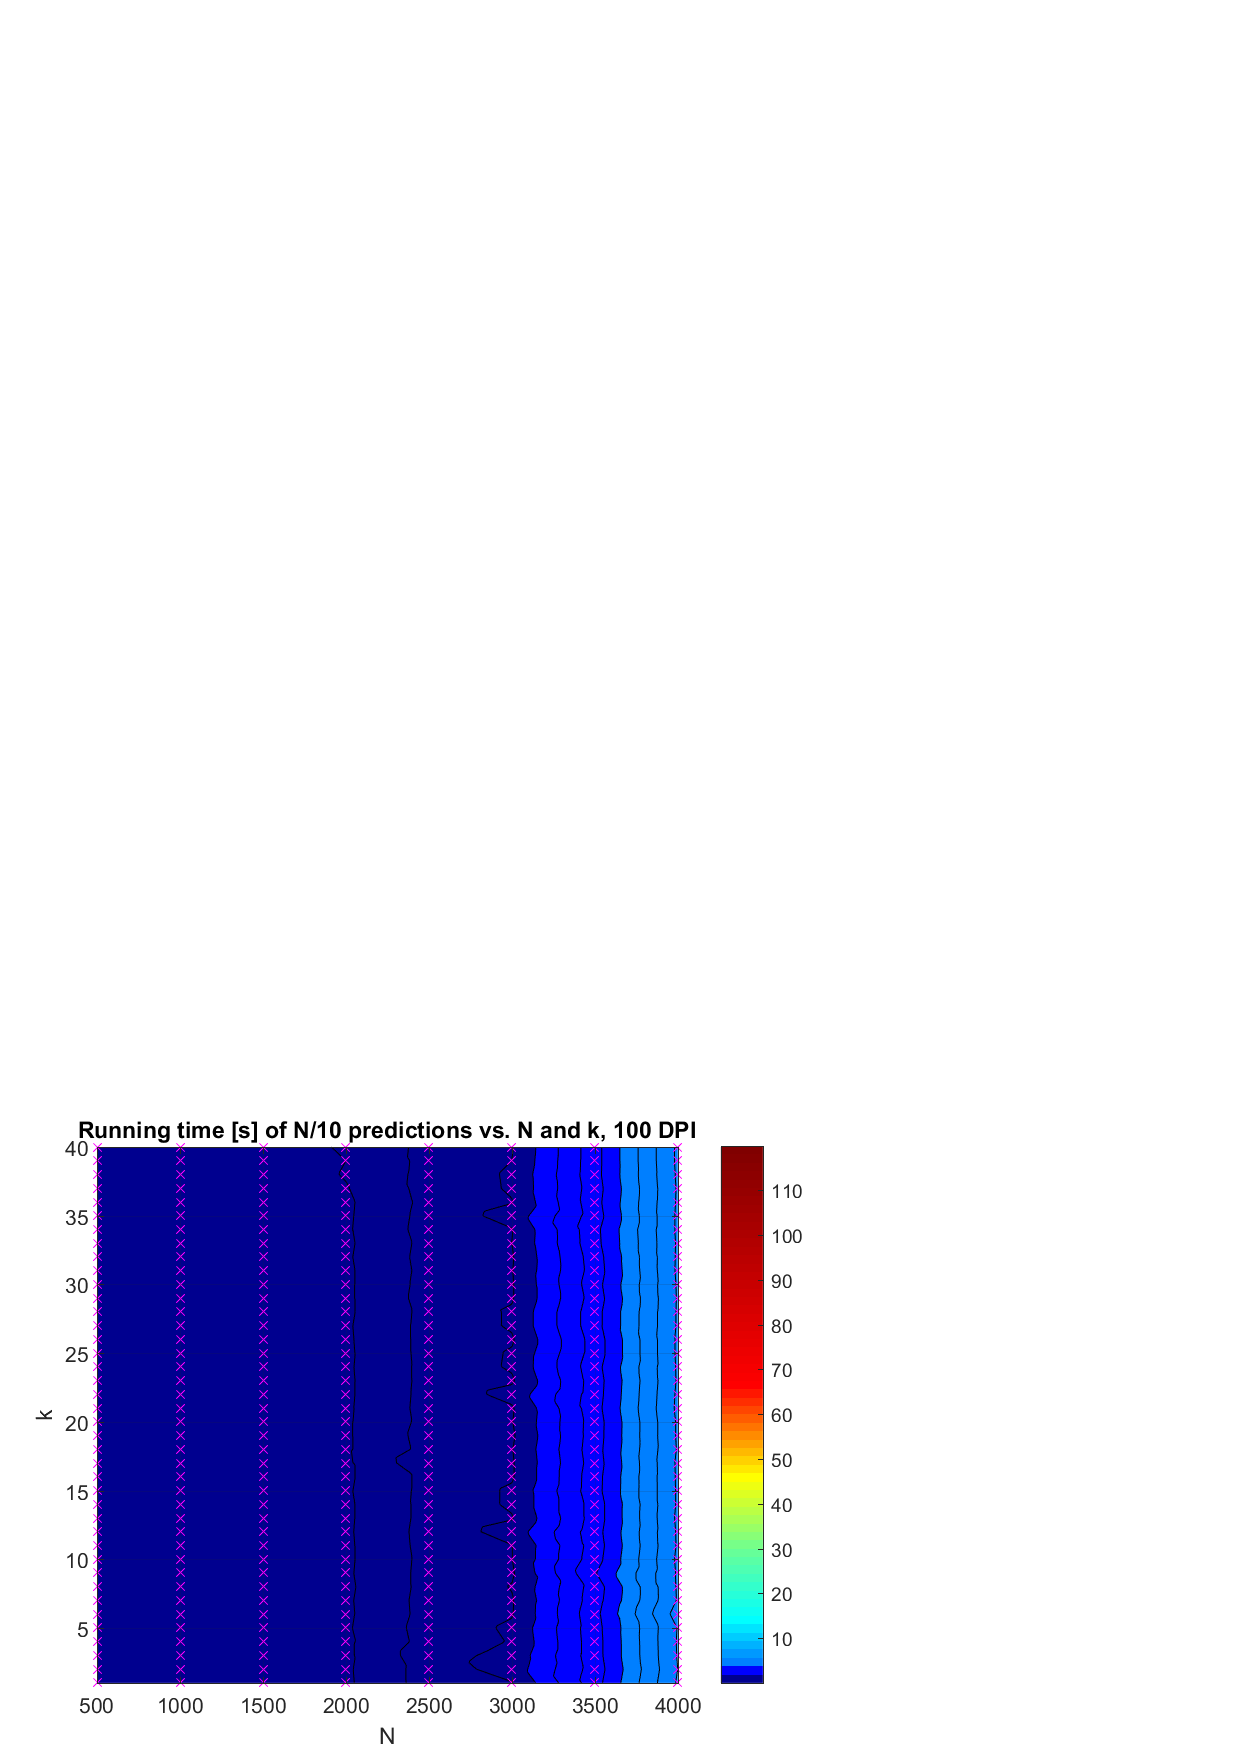
\includegraphics[width = \textwidth]{graphics/knn-runningtime-vs-n-and-k-2-2-dpi100}
		\caption{100 DPI}
	\end{subfigure}
	\begin{subfigure}[t]{0.33\textwidth}
		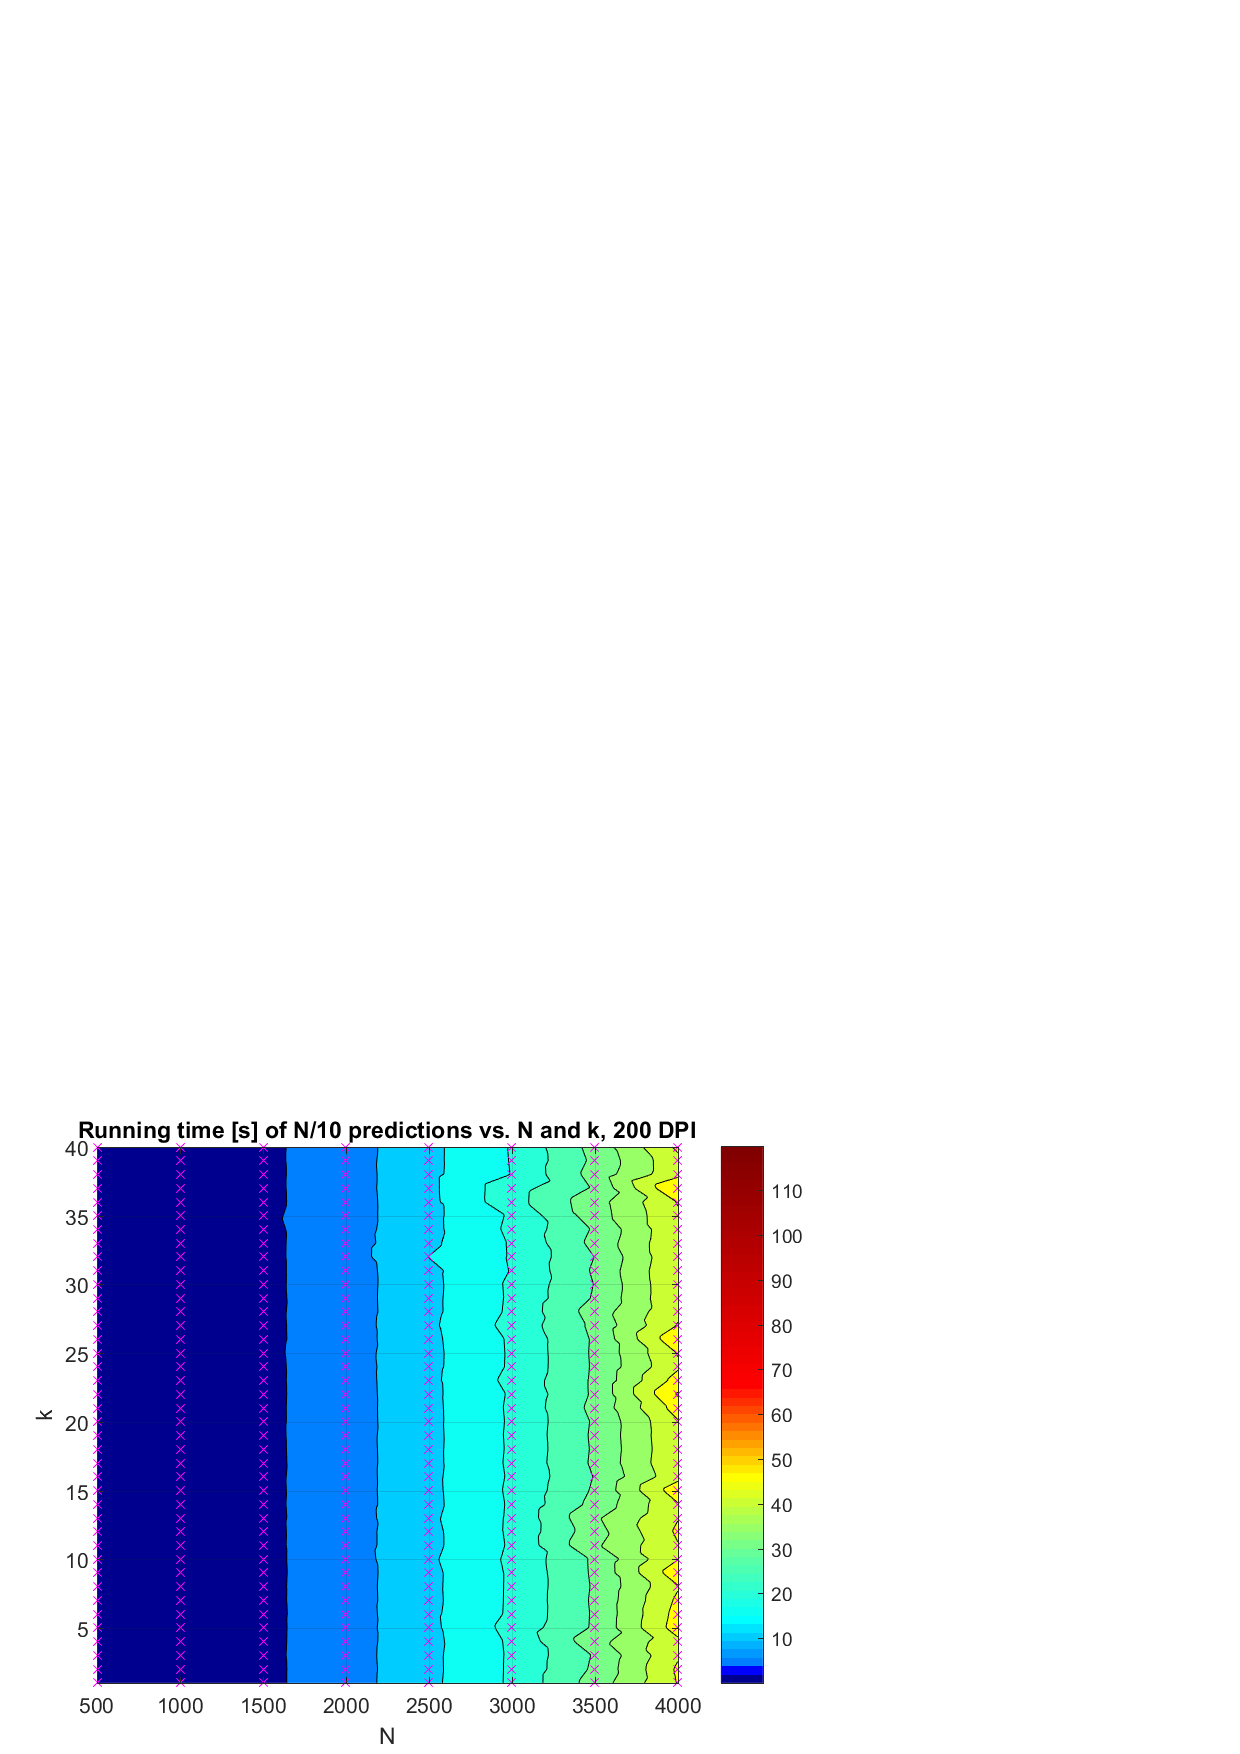
\includegraphics[width = \textwidth]{graphics/knn-runningtime-vs-n-and-k-2-2-dpi200}
		\caption{200 DPI}
	\end{subfigure}
	\begin{subfigure}[t]{0.33\textwidth}
		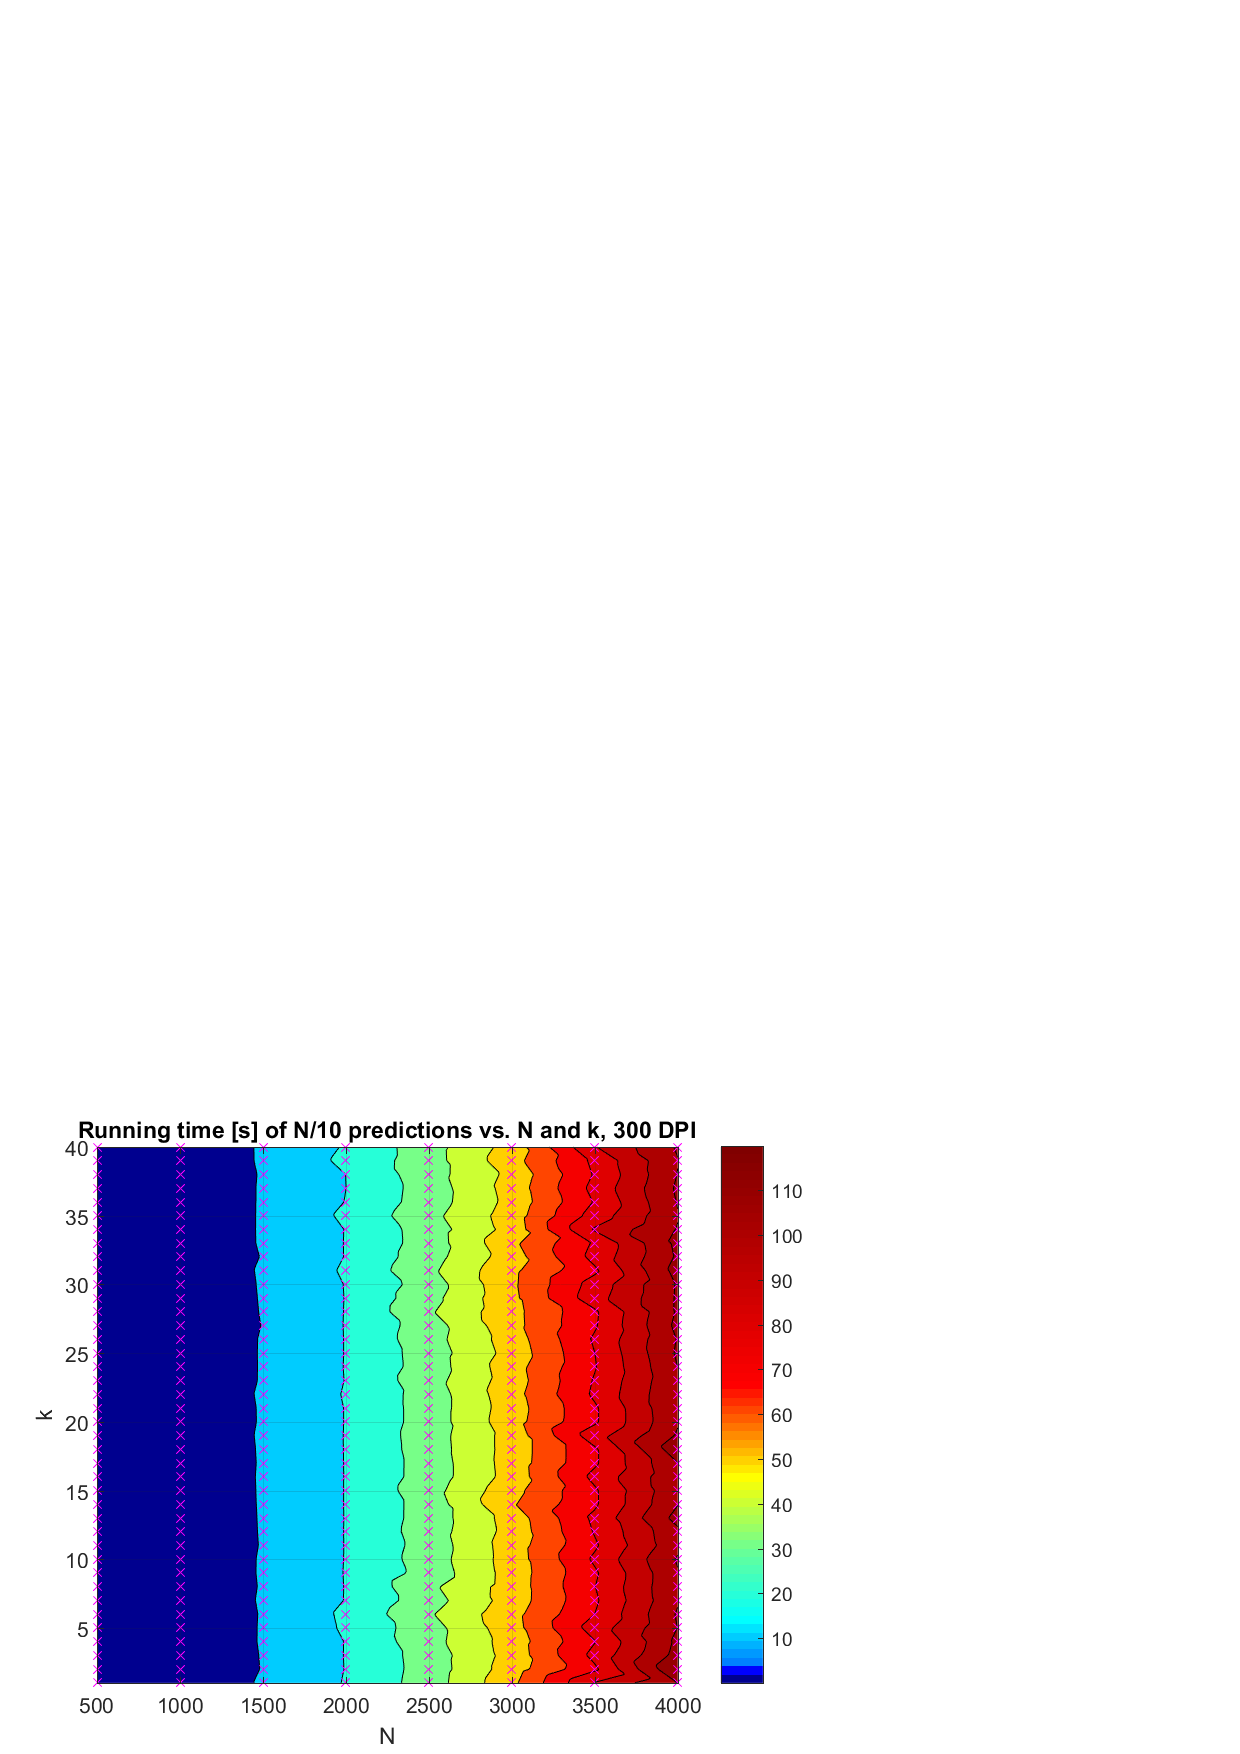
\includegraphics[width = \textwidth]{graphics/knn-runningtime-vs-n-and-k-2-2-dpi300}
		\caption{300 DPI}
	\end{subfigure}
	\caption{
		k-NN prediction running time in seconds
		vs. dataset size N and k for G2M2 data at various DPI.
		}
	\label{fig:knn-runningtime-vs-n-and-k}
\end{figure}

It is clearly seen that running times are much reduced by downsampling,
and that running times increase substantially with N. It is also seen that
the running times do not vary with k.
Figure \ref{fig:knn-runningtime-vs-n-loglog} visualizes the relationship
between running time and N further.
\begin{figure}[ht]
	\centering
	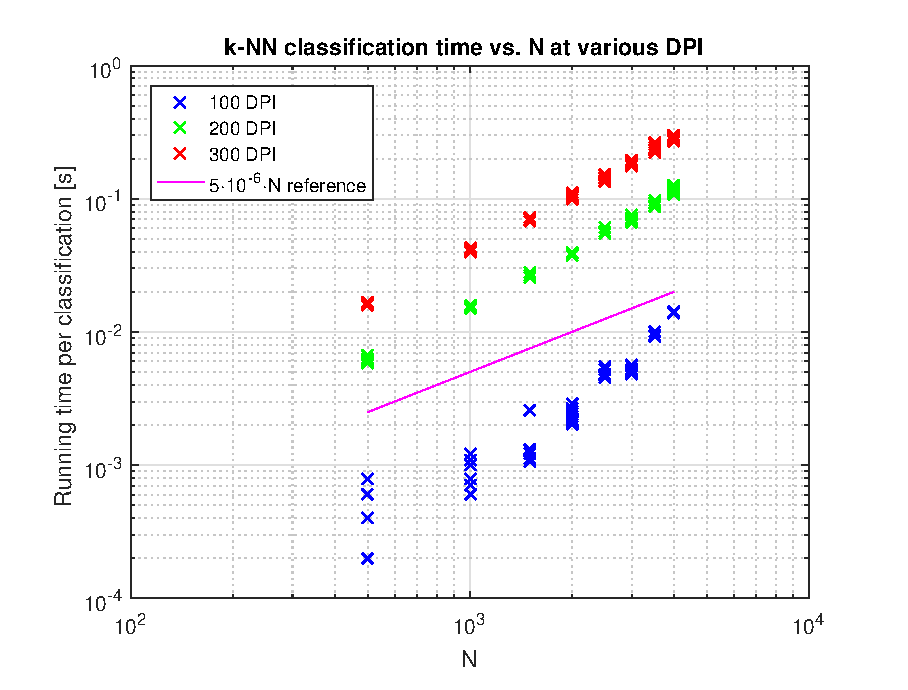
\includegraphics[width = 0.5\textwidth]{graphics/knn-runningtime-vs-n-loglog-2-2}
	\caption{
		log-log plot of k-NN prediction running time in seconds vs. N at various DPI.
		\(5\cdot{}10^{-6}\cdot{}N\) reference also plotted.
	}
	\label{fig:knn-runningtime-vs-n-loglog}
\end{figure}

It can be seen from figure \ref{fig:knn-runningtime-vs-n-loglog} that
the classification time complexity is larger than \(O(N)\).

These results indicate that the entire dataset is sorted and searched through for
each classification, and that this type of problem does not scale well with increasing
dataset size.
Since methods are to be compared with data from several individuals,
it was therefore chosen to use 100 DPI downsampling for further data processing,
at the cost of classification accuracy (as found in the first exercise).
